% ---------------------------------------------------------------------------- %

\section{Planeamento do Projeto}
\label{cap:planeamento}

Estando fundamentada a construção do assistente \emph{Bela Sopa}, apresenta-se agora o planeamento do seu desenvolvimento. Começa-se por se definir um modelo inicial do sistema, procedendo-se com a identificação de recursos necessários à sua concretização e de medidas de sucesso. Por fim, apresenta-se um plano cronológico detalhado do seu desenvolvimento.

% ---------------------------------------------------------------------------- %

\subsection{Maqueta do sistema}
\label{cap:planeamento:maqueta}

Embora não seja ainda possível determinar o conjunto exato de funcionalidades desejadas e a estrutura interna do sistema a ser desenvolvido, podem já ser identificados os seus principais tipos de utilizador e componentes, assim como possíveis dependências em serviços externos.

\begin{figure}[ht]
  \centering
  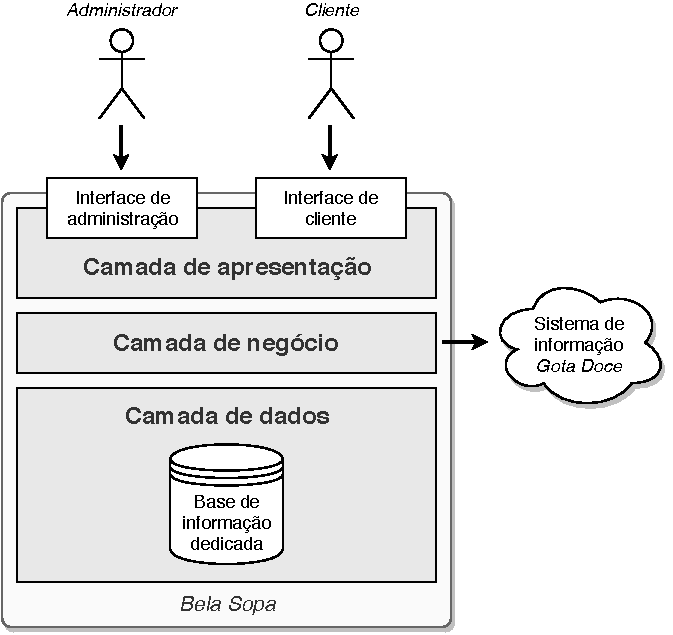
\includegraphics{figures/03/maqueta.pdf}
  \caption{Maqueta do sistema.}
  \label{fig:planeamento:maqueta}
\end{figure}

Com base nessa informação, foi elaborado um modelo inicial do sistema (ou \emph{maqueta}), o qual é apresentado na \reffig{fig:planeamento:maqueta}. Identificam-se dois tipos de utilizador: \emph{administradores} --- responsáveis pela gestão dos conteúdos disponibilizados --- e \emph{clientes} --- correspondentes ao público-alvo do sistema \emph{Bela Sopa}. Na figura, a entidade ou componente na origem de cada seta inicia interações com o componente no destino da mesma.

Prevê-se a possibilidade de a plataforma fazer uso de um sistema de informação detido pela empresa \emph{Gota Doce} por forma a obter dados sobre produtos e lojas da mesma e a tirar partido da base de informação relativa a receitas culinárias e ingredientes atualmente em uso pelo serviço \emph{Escola de Cozinha}. No entanto, prevê-se também que a plataforma necessite de uma base de informação própria, dedicada à gestão de dados específicos ao serviço a ser desenvolvido.

Explicita-se que este modelo é provisório e não vinculativo, tendo o principal objetivo de auxiliar a identificação de recursos necessários ao desenvolvimento do sistema e o início da fase de especificação do mesmo.

% ---------------------------------------------------------------------------- %

\subsection{Recursos necessários}
\label{sec:planeamento:recursos}

%\begin{itemize}
%  \item Não é ``computadores e software''.
%  \item Recursos importantes para garantir o %sucesso do desenvolvimento do sistema.
%  \item Equipa de desenvolvimento.
%  \item E equipa que nos dá o conhecimento %necessário (em culinária).
%\end{itemize}

Estabeleceu-se que, para o desenvolvimento do sistema, é necessária uma equipa de desenvolvimento de 8 elementos, respetivamente, 1 gestor, 1 analista, 4 programadores e 2 engenheiros de software.

Para além disso, será necessário utilizar os recursos disponibilizados pela empresa \emph{Gota Doce}, como a base de receitas da plataforma \emph{Escola de Cozinha}, por forma a obter o nome das receitas, a dificuldade, a duração, os ingredientes, os passos da receita e as porções concebidas para as sopas, e um consultor que nos dará a informação necessária sobre culinária.

% ---------------------------------------------------------------------------- %

\subsection{Medidas de sucesso}
\label{sec:planeamento:medidas-sucesso}

% \alberto{Sugestão: Ter \textbf{\emph{lista}} de medidas de sucesso sucintas, objetivas e quantitativas.}

As medidas de sucesso aqui enumeradas foram estabelecidas através de uma reunião entre o nosso gestor e a equipa de contabilidade do nosso cliente, sendo que os dados referidos foram especulados com base em 6 meses de uso do sistema após o seu lançamento.

Estima-se que:

\begin{itemize}
    
    \item A venda de produtos aumente em, pelo menos, 5\% através da utilização do sistema;
    
    \item O sistema seja utilizado em média por 1000 utilizadores distintos por dia;
    
    \item O número de clientes da cadeia aumente em, pelo menos, 3\%;
    
    % \item Assegure os clientes atuais que estão bem servidos;
    
    % \item Um aumento 10\% na procura de produtos e 5\% nos pedidos via online que por consequente aumenta 3\% a utilização do serviço entrega ao domicílio.

    \item O número de pedidos efetuados através do serviço de entrega ao domicílio aumente em, pelo menos, 10\%.

\end{itemize}

% ---------------------------------------------------------------------------- %

\subsection{Plano de desenvolvimento}
\label{sec:planeamento:plano-desenvolvimento}

% \begin{itemize}
%   \item Diagrama de Gantt -- Microsoft Project.
%   \item Distribuição de trabalho por pessoa? (???)
%   \item Quantidade de horas de trabalho.
%   \item Assumir trabalhar ao dia, dias de 8 horas.
%   \item Dá depois para contabilizar o quanto vamos gastar a desenvolver o projeto ("era engraçado fazerem isso").
%   \item E.g.: contabilizar tempo para falar com consultor (por exemplo, chef). Uma semana chega, faz de conta, e vamos levar 2 pessoas para falar.
%   \item Convém manter Gantt original no relatório final.
% \end{itemize}

\begin{figure}[ht]
  \centering
  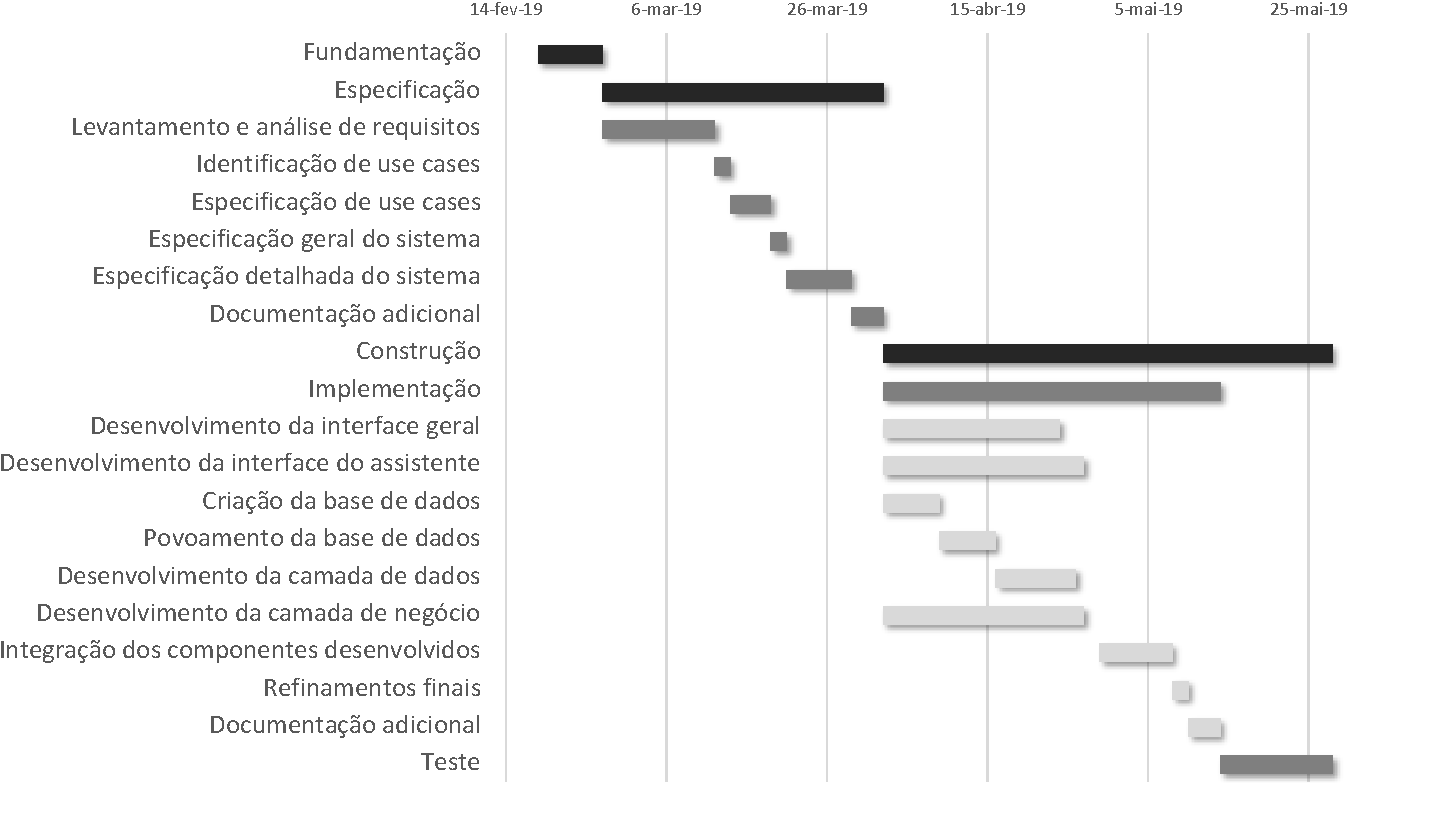
\includegraphics[width=\textwidth]{figures/03/planeamento-gantt.pdf}
  \caption{Diagrama de Gantt para o desenvolvimento do projeto.}
  \label{fig:planeamento:gantt}
\end{figure}

A análise e fundamentação do projeto será feita pelo analista da equipa, e os restantes processos só serão feitos após esta fase, com uma duração de 6 dias.

Durante o desenvolvimento do sistema estimam-se 6 tarefas necessárias, respetivamente, levantamento de requisitos, análise de requisitos, arquitetura de software, testes e implementação.
O gestor e os colaboradores correspondentes à fase atual do projeto, irão se reunir duas vezes por semana de forma a distribuir tarefas para permitir trabalho autónomo e debater eventuais dúvidas, conflitos ou problemas no trabalho a realizar.

O levantamento de requisitos e sua respetiva análise terá a duração de 3 dias e será realizado pelos engenheiros de software e com o auxilio de um consultor ainda a ser disponibilizado pelo \emph{Gota Doce}.

A identificação e especificação de use cases demorará 4 dias e será feito após o levantamento e análise de requisitos. A arquitetura de software terá um espaço de 4 semanas e será realizada pelos engenheiros de software. A implementação terá a duração de 6 semanas e será realizada pelos programadores.

Os testes serão feitos durante 10 dias por um programador da equipa de desenvolvimento e um outro programador que desconhece o produto, de forma a que os testes sejam feitos de forma imparcial e independentes do facto do colaborador ter desenvolvido o produto ou não. Após isto, durante 4 dias será realizada a apresentação e instalação do sistema de software nos ambientes do cliente.

Em suma, estimam-se 14 semanas para o desenvolvimento deste sistema.

O custo associado a cada uma das fases do projeto encontra-se na Figura \ref{fig:planeamento:custosgerais}, estando associado ao custo inicial a fase "Análise e fundamentação". Em suma o custo total do projeto é de 30.052,00 euros.

\begin{figure}[ht]
  \centering
  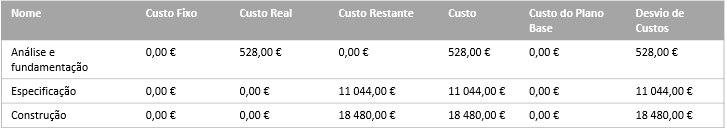
\includegraphics[width=\textwidth]{figures/03/planeamento-custos.png}
  \caption{Custos associados a cada fase do projeto.}
  \label{fig:planeamento:custosgerais}
\end{figure}

Estes custos foram gerados tendo em conta 8 horas de trabalho por dia, 5 dias por semana, e os custos para cada elemento individualmente que se encontram na \reffig{fig:planeamento:recursoshumanos}.

\begin{figure}[ht]
  \centering
  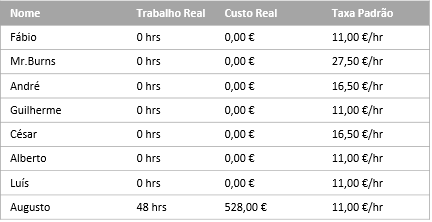
\includegraphics[scale=1.15]{figures/03/planeamento-recursos.png}
  \caption{Custos associados a cada contribuidor do projeto.}
  \label{fig:planeamento:recursoshumanos}
\end{figure}

% ---------------------------------------------------------------------------- %
